\documentclass[border=10pt]{standalone}
\usepackage{pgfplots}
\pgfplotsset{compat=1.18}
\begin{document}
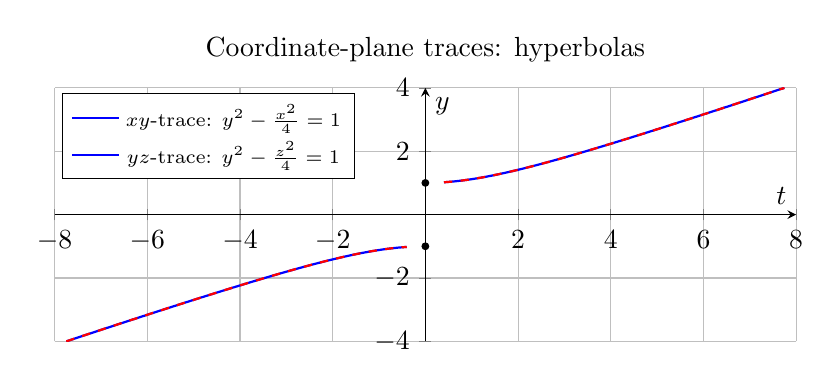
\begin{tikzpicture}
\begin{axis}[
    width=11cm,
    height=4.8cm,
    xlabel={$t$},
    ylabel={$y$},
    title={Coordinate-plane traces: hyperbolas},
    xmin=-8, xmax=8,
    ymin=-4, ymax=4,
    axis lines=middle,
    grid=major,
    legend style={at={(0.01,0.98)}, anchor=north west, font=\scriptsize},
]
\addplot[domain=-4:-1.02, samples=120, thick, blue] ({-2*sqrt(x^2-1)}, {x});
\addplot[domain=1.02:4, samples=120, thick, blue] ({2*sqrt(x^2-1)}, {x});
\addlegendentry{$xy$-trace: $y^2-\frac{x^2}{4}=1$}
\addplot[domain=-4:-1.02, samples=120, thick, red, dashed] ({-2*sqrt(x^2-1)}, {x});
\addplot[domain=1.02:4, samples=120, thick, red, dashed] ({2*sqrt(x^2-1)}, {x});
\addlegendentry{$yz$-trace: $y^2-\frac{z^2}{4}=1$}
\addplot[only marks, mark=*, mark size=1.2pt, black] coordinates {(0,1) (0,-1)};
\end{axis}
\end{tikzpicture}
\end{document}